%  A simple AAU report template.
%  2015-05-08 v. 1.2.0
%  Copyright 2010-2015 by Jesper Kjær Nielsen <jkn@es.aau.dk>
%
%  This is free software: you can redistribute it and/or modify
%  it under the terms of the GNU General Public License as published by
%  the Free Software Foundation, either version 3 of the License, or
%  (at your option) any later version.
%
%  This is distributed in the hope that it will be useful,
%  but WITHOUT ANY WARRANTY; without even the implied warranty of
%  MERCHANTABILITY or FITNESS FOR A PARTICULAR PURPOSE.  See the
%  GNU General Public License for more details.
%
%  You can find the GNU General Public License at <http://www.gnu.org/licenses/>.
%
%  A simple AAU report template.
%  2015-05-08 v. 1.2.0
%  Copyright 2010-2015 by Jesper Kjær Nielsen <jkn@es.aau.dk>
%
%  This is free software: you can redistribute it and/or modify
%  it under the terms of the GNU General Public License as published by
%  the Free Software Foundation, either version 3 of the License, or
%  (at your option) any later version.
%
%  This is distributed in the hope that it will be useful,
%  but WITHOUT ANY WARRANTY; without even the implied warranty of
%  MERCHANTABILITY or FITNESS FOR A PARTICULAR PURPOSE.  See the
%  GNU General Public License for more details.
%
%  You can find the GNU General Public License at <http://www.gnu.org/licenses/>.
%
\documentclass[12pt,twoside,a4paper,openright]{report}
%%%%%%%%%%%%%%%%%%%%%%%%%%%%%%%%%%%%%%%%%%%%%%%%
% Language, Encoding and Fonts
% http://en.wikibooks.org/wiki/LaTeX/Internationalization
%%%%%%%%%%%%%%%%%%%%%%%%%%%%%%%%%%%%%%%%%%%%%%%%
% Select encoding of your inputs. Depends on
% your operating system and its default input
% encoding. Typically, you should use
%   Linux  : utf8 (most modern Linux distributions)
%            latin1 
%   Windows: ansinew
%            latin1 (works in most cases)
%   Mac    : applemac
% Notice that you can manually change the input
% encoding of your files by selecting "save as"
% an select the desired input encoding. 
\usepackage[utf8]{inputenc}
% Make latex understand and use the typographic
% rules of the language used in the document.
\usepackage[danish,english]{babel}
% Use the palatino font
\usepackage[sc]{mathpazo}
\linespread{1.05}         % Palatino needs more leading (space between lines)
% Choose the font encoding
\usepackage[T1]{fontenc}
%%%%%%%%%%%%%%%%%%%%%%%%%%%%%%%%%%%%%%%%%%%%%%%%
% Graphics and Tables
% http://en.wikibooks.org/wiki/LaTeX/Importing_Graphics
% http://en.wikibooks.org/wiki/LaTeX/Tables
% http://en.wikibooks.org/wiki/LaTeX/Colors
%%%%%%%%%%%%%%%%%%%%%%%%%%%%%%%%%%%%%%%%%%%%%%%%
% load a colour package
\usepackage[table,xcdraw]{xcolor}
\definecolor{aaublue}{RGB}{33,26,82}% dark blue
% The standard graphics inclusion package
\usepackage{graphicx}
% Set up how figure and table captions are displayed
\usepackage{caption}
\captionsetup{%
  font=footnotesize,% set font size to footnotesize
  labelfont=bf % bold label (e.g., Figure 3.2) font
}
% Make the standard latex tables look so much better
\usepackage{array,booktabs}
% Enable the use of frames around, e.g., theorems
% The framed package is used in the example environment
\usepackage{framed}

%%%%%%%%%%%%%%%%%%%%%%%%%%%%%%%%%%%%%%%%%%%%%%%%
% Mathematics
% http://en.wikibooks.org/wiki/LaTeX/Mathematics
%%%%%%%%%%%%%%%%%%%%%%%%%%%%%%%%%%%%%%%%%%%%%%%%
% Defines new environments such as equation,
% align and split 
\usepackage{amsmath}
% Adds new math symbols
\usepackage{amssymb}
% Use theorems in your document
% The ntheorem package is also used for the example environment
% When using thmmarks, amsmath must be an option as well. Otherwise \eqref doesn't work anymore.
\usepackage[framed,amsmath,thmmarks]{ntheorem}

%%%%%%%%%%%%%%%%%%%%%%%%%%%%%%%%%%%%%%%%%%%%%%%%
% Algorithms (including pseudocode)
% https://en.wikibooks.org/wiki/LaTeX/Algorithms
%%%%%%%%%%%%%%%%%%%%%%%%%%%%%%%%%%%%%%%%%%%%%%%%
% Defines the environment algorithm
% which should be used to show line numbers
\usepackage{algorithm}

% Defines the environment algorithmic
% and the commands used herein
\usepackage[noend]{algpseudocode}

% Setup for algorithmic
\algrenewcommand\alglinenumber[1]{\textit{\scriptsize #1.}}
%\renewcommand{\COMMENT}[2][.5\linewidth]{%
%  \leavevmode\hfill\makebox[#1][l]{//~#2}}
\renewcommand{\algorithmiccomment}[1]{\leavevmode\hfill\makebox[.5\linewidth][l]{//~#1}}
\algnewcommand\In{\textbf{in }}
\algnewcommand\Where{\textbf{where }}
\algnewcommand\Or{\textbf{or }}
\algnewcommand\AND{\textbf{and }}
\algnewcommand\True{\textbf{true }}

%%%%%%%%%%%%%%%%%%%%%%%%%%%%%%%%%%%%%%%%%%%%%%%%
% Page Layout
% http://en.wikibooks.org/wiki/LaTeX/Page_Layout
%%%%%%%%%%%%%%%%%%%%%%%%%%%%%%%%%%%%%%%%%%%%%%%%
% Change margins, papersize, etc of the document
\usepackage[
  inner=28mm,% left margin on an odd page
  outer=41mm,% right margin on an odd page
  ]{geometry}
% Modify how \chapter, \section, etc. look
% The titlesec package is very configureable
\usepackage{titlesec}
\titleformat{\chapter}
{\normalfont\Huge\bfseries}{\filright\thechapter}
{20pt}{\Huge\filright}
\titleformat*{\section}{\normalfont\Large\bfseries}
\titleformat*{\subsection}{\normalfont\large\bfseries}
\titleformat*{\subsubsection}{\normalfont\normalsize\bfseries}
%\titleformat*{\paragraph}{\normalfont\normalsize\bfseries}
%\titleformat*{\subparagraph}{\normalfont\normalsize\bfseries}

% Clear empty pages between chapters
\let\origdoublepage\cleardoublepage
\newcommand{\clearemptydoublepage}{%
  \clearpage
  {\pagestyle{empty}\origdoublepage}%
}
\let\cleardoublepage\clearemptydoublepage

% Change the headers and footers
\usepackage{fancyhdr}
\pagestyle{fancy}
\fancyhf{} %delete everything
\renewcommand{\headrulewidth}{0pt} %remove the horizontal line in the header
\fancyhead[RE]{\small\nouppercase\leftmark} %even page - chapter title
\fancyhead[LO]{\small\nouppercase\rightmark} %uneven page - section title
\fancyhead[LE,RO]{\thepage} %page number on all pages
% Do not stretch the content of a page. Instead,
% insert white space at the bottom of the page
\raggedbottom
% Enable arithmetics with length. Useful when
% typesetting the layout.
\usepackage{calc}

%%%%%%%%%%%%%%%%%%%%%%%%%%%%%%%%%%%%%%%%%%%%%%%%
% Bibliography
% http://en.wikibooks.org/wiki/LaTeX/Bibliography_Management
%%%%%%%%%%%%%%%%%%%%%%%%%%%%%%%%%%%%%%%%%%%%%%%%
\usepackage[backend=bibtex,
  bibencoding=utf8
  ]{biblatex}
\addbibresource{bib/mybib}

%%%%%%%%%%%%%%%%%%%%%%%%%%%%%%%%%%%%%%%%%%%%%%%%
% Misc
%%%%%%%%%%%%%%%%%%%%%%%%%%%%%%%%%%%%%%%%%%%%%%%%
\usepackage{listings}
\usepackage{listings, color}
% Add bibliography and index to the table of
% contents
\usepackage[nottoc]{tocbibind}
\usepackage{svg}
% Add the command \pageref{LastPage} which refers to the
% page number of the last page
\usepackage{lastpage}
% Add todo notes in the margin of the document
\usepackage[
%  disable, %turn off todonotes
  colorinlistoftodos, %enable a coloured square in the list of todos
  textwidth=\marginparwidth, %set the width of the todonotes
  textsize=scriptsize, %size of the text in the todonotes
  ]{todonotes}

%%%%%%%%%%%%%%%%%%%%%%%%%%%%%%%%%%%%%%%%%%%%%%%%
% Hyperlinks
% http://en.wikibooks.org/wiki/LaTeX/Hyperlinks
%%%%%%%%%%%%%%%%%%%%%%%%%%%%%%%%%%%%%%%%%%%%%%%%
% Enable hyperlinks and insert info into the pdf
% file. Hypperref should be loaded as one of the 
% last packages
\usepackage{hyperref}
\hypersetup{%
	plainpages=false,%
	pdfauthor={Author(s)},%
	pdftitle={Title},%
	pdfsubject={Subject},%
	bookmarksnumbered=true,%
	colorlinks=false,%
	citecolor=black,%
	filecolor=black,%
	linkcolor=black,% you should probably change this to black before printing
	urlcolor=black,%
	pdfstartview=FitH%
}

\definecolor{forestgreen}{RGB}{34,139,34}
\definecolor{orangered}{RGB}{239,134,64}
\definecolor{darkblue}{rgb}{0.0,0.0,0.6}
\definecolor{gray}{rgb}{0.4,0.4,0.4}

\lstdefinestyle{XML} {
    belowcaptionskip=1\baselineskip,
    captionpos=b,
    language=XML,
    extendedchars=true, 
    breaklines=true,
    breakatwhitespace=true,
    emph={},
    emphstyle=\color{red},
    basicstyle=\ttfamily,
    columns=fullflexible,
    commentstyle=\color{gray}\upshape,
    morestring=[b]",
    morecomment=[s]{<?}{?>},
    morecomment=[s][\color{forestgreen}]{<!--}{-->},
    keywordstyle=\color{orangered},
    stringstyle=\ttfamily\color{black}\normalfont,
    tagstyle=\color{darkblue}\bf,
    morekeywords={id,attribute,xmlns,version,type,release, uid, user, key, value, changeset, longitude, latitude, timestamp},
}

\lstdefinestyle{java}{
  language=Java,
  captionpos=b,
  aboveskip=3mm,
  belowskip=3mm,
  showstringspaces=false,
  columns=flexible,
  basicstyle={\footnotesize\ttfamily},
  numberstyle={\tiny},
  numbers=left,
  keywordstyle=\color{blue},
  commentstyle=\color{dkgreen},
  stringstyle=\color{mauve},
  breaklines=true,
  breakatwhitespace=true,
  tabsize=3
}
\lstset{
  literate={"}{\textquoteright\textquoteright}1
}
\usepackage{qtree}
\theoremstyle{definition}
\newtheorem{exmp}{Example}[section]
\makeatletter
\newcommand{\thickhline}{%
	\noalign {\ifnum 0=`}\fi \hrule height 1pt
	\futurelet \reserved@a \@xhline
}
\newcolumntype{T}{|@{}|@{}|}
\makeatother
% package inclusion and set up of the document
\input{setup/hyphenations.tex}% 
\input{setup/macros.tex}% my new macros

\begin{document}
%frontmatterf
\pagestyle{empty} %disable ers and footers
\pagenumbering{roman} %use roman page numbering in the frontmatter
\input{sections/frontpage.tex}
\input{sections/colophon.tex}
\pdfbookmark[0]{English title page}{label:titlepage_en}
\aautitlepage{%
  \englishprojectinfo{
    Less obstructed street traffic%title
  }{%
    Intelligent or Massively Parallel Systems %theme
  }{%
    Fall Semester 2015 %project period
  }{%
    d505e15 % project group
  }{%
    %list of group members
    Andreas Hairing Klostergaard\\
    Benjamin Ahm\\
    Kristian Hauge Jensen\\
    Michael Jensen\\
    Morten Rune Peterson\\
    Morten Korsholm Terndrup
  }{%
    %list of supervisors
    Bin Yang
  }{%
    3 % number of printed copies
  }{%
    \today % date of completion
  }%
}{%department and address
  \textbf{Department of Computer Science}\\
  Aalborg University\\
  Selma Lagerlöfsvej 300\\
  9000 Aalborg\\
  \href{http://www.aau.dk}{http://www.aau.dk}
}{% the abstract
This report looks at the possibility of using machine intelligence and distributed systems to gather and analyse traffic data. The main focus of this project is machine intelligence where distributed systems is a support part. The system need to split up traffic so the route network is better utilise. A lot of software used in this project is not made by the group, but taken from other free or open sours projects because these elements is not the focus of this project.
}

\cleardoublepage
%{\selectlanguage{danish}
%\pdfbookmark[0]{Danish title page}{label:titlepage_da}
%\aautitlepage{%
%  \danishprojectinfo{
%    Rapportens titel %title
%  }{%
%    Semestertema %theme
%  }{%
%    Efterårssemestret 2010 %project period
%  }{%
%    XXX % project group
%  }{%
%    %list of group members
%    Forfatter 1\\
%    Forfatter 2\\
%    Forfatter 3
%  }{%
%    %list of supervisors
%    Vejleder 1\\
%    Vejleder 2
%  }{%
%    1 % number of printed copies
%  }{%
%    \today % date of completion
%  }%
%}{%department and address
%  \textbf{Elektronik og IT}\\
%  Aalborg Universitet\\
%  \href{http://www.aau.dk}{http://www.aau.dk}
%}{% the abstract
%  Her er resuméet
%}}

\cleardoublepage
\pdfbookmark[0]{Contents}{label:contents}
\pagestyle{fancy} %enable headers and footers again
\setcounter{tocdepth}{1}
\tableofcontents
\listoftodos
\chapter*{Preface\markboth{Preface}{Preface}}\label{ch:preface}
\addcontentsline{toc}{chapter}{Preface}
This report is part of a 5th semester project at Aalborg University. The purpose of the project is to achieve a set of learning goals specified by the study regulation for Computer Science bachelors degree\todo{source}. More specifically, the goal is to achieve knowledge, skills and competencies within the fields of Machine Intelligence, which is the primary focus of this project.

Since not all project group members are following the optional machine intelligence course, machine learning techniques are supported by Distributed Systems and Network techniques. The reason for this is to also achieve knowledge, skills and competencies about this field as well since this is important for some of the group members.

%We believe we have achieved the goals of the study regulation through the work documented in the report. We have achieved knowledge, skills and competencies about different machine learning techniques through the analysis, implementation and evaluation of the techniques for learning traffic patterns.
 
We would like to extend our thanks to Fabrice Marchal and TrackMatching for being helpful and providing increased quotas for their map-matching service.

\vspace{\baselineskip}\hfill Aalborg University, \today
\vfill\noindent
\begin{minipage}[b]{0.45\textwidth}
 \centering
 \rule{\textwidth}{0.5pt}\\
  Andreas Hairing Klostergaard\\
 {\footnotesize <aklost11@student.aau.dk>}
\end{minipage}
\hfill
\begin{minipage}[b]{0.45\textwidth}
 \centering
 \rule{\textwidth}{0.5pt}\\
  Benjamin Ahm\\
 {\footnotesize <bahm13@student.aau.dk>}
\end{minipage}

\vspace{3\baselineskip}\noindent
\begin{minipage}[b]{0.45\textwidth}
 \centering
 \rule{\textwidth}{0.5pt}\\
  Kristian Hauge Jensen\\
 {\footnotesize <kje13@student.aau.dk>}
\end{minipage}
\hfill
\begin{minipage}[b]{0.45\textwidth}
 \centering
 \rule{\textwidth}{0.5pt}\\
  Michael Jensen\\
 {\footnotesize <mj09@student.aau.dk>}
\end{minipage}

\vspace{3\baselineskip}\noindent
\begin{minipage}[b]{0.45\textwidth}
 \centering
 \rule{\textwidth}{0.5pt}\\
  Morten Rune Peterson\\
 {\footnotesize <mopete13@student.aau.dk>}
\end{minipage}
\hfill
\begin{minipage}[b]{0.45\textwidth}
 \centering
 \rule{\textwidth}{0.5pt}\\
  Morten Korsholm Terndrup\\
 {\footnotesize <mternd13@student.aau.dk>}
\end{minipage}

\cleardoublepage
%mainmatter
\pagenumbering{arabic} %use arabic page numbering in the mainmatter
\chapter{Introduction}\label{chap:introduction}

Transportation problems arise frequently in areas with high population density. It has been estimated that the total number of vehicles in the world will have increased by more than 150\% between 2002 and 2030\cite{dargay2007vehicle}, which will in all likelihood aggravate the current transportation problems. Many of these problems become accentuated when notable events occur, such as concerts, holidays, and traffic accidents.

This report explores these problems, formalizes them, and proposes a solution that uses machine intelligence(MI) and distributed systems to alleviate them.\todo{Rewrite with smoother mentions of MI and DSN.} This raises the question ``can the study of MI and distributed systems help in solving this increasing load on the road network?''. This could be by smarter use of the road network or by making a driving plan fx. so all people don't drive to or from work at the same time. These are just some possibly solutions ideas, but a deeper understanding of this two areas of computer science are need to know if this is possible.
\todo{Move some/all of the previous introduction to "Relevance" and/or merge with the current introduction.}

%Transportation problems arise frequently in areas with high population density. Examples that come to mind are people standing in line for services, traffic congestion on roads, and overcrowded public transportation. Many of these problems become accentuated when notable events occur, such as concerts, people going on holidays, and traffic accidents. Designing an infrastructure with these potential problems in mind can certainly minimize the troubles they cause. However, infrastructures are typically designed with a particular context in mind and consequently do not respond well to serious changes in the area, such as an increasing number of people. Costs are high when roads have to be expanded, changed, or constructed, and maintenance costs increase as roads more regularly need to be renewed when the everyday traffic in the area increases. For these reasons, it is advantageous to achieve better utilisation of road networks, such that costs of overburdened roads can be lowered as well as saving time for the people stuck in traffic congestions. This leads to an initial problem for this project: How can we analyse traffic to detect current and possibly future problems, such that initiatives for alleviating them can be considered.\todo{Læs intro. Måske nogle ting her, der tilhører relevans. Skal vi havde noget med hvordan det påvirker folk physik}

% Problem analysis
\chapter{Problem analysis}
[here is the intro for the problem analysis]
\section{Relevance}
Traffic problems have several consequences and affect several different groups of people and organizations. Estimates show that the number of cars in the world is increasing year by year\cite{WardsAuto:CarPopulation}. This increase can potentially lead to an increase in traffic congestions, which in turn increases the need for better infrastructure or more efficient traffic flow.

% wear on roads
Likewise, many of the roads that are congested are heavily used roads. These roads see more wear than less used roads and therefore requires either special construction or more maintenance, which increases the costs for governments on infrastructure. Maintenance of roads also obstructs the road network, since parts of a road can be unavailable which can result in temporarily slower traffic.

% Emissions
Another issue that is a consequence of traffic congestion is the increased CO2-emissions of vehicles frequently accelerating and decelerating in a congested area\cite{BarthBoriboonsomsin2009}.

% Time wasted --> stress
Being stuck in traffic can also affect the well-being of drivers as stress levels increase. A study of the relationship between traffic congestion and driver stress observes that there is a correlation between drivers' stressed behaviour and the traffic situation\cite{HennesyWiesenthal1997,StokolsNovacoStokolsCampell1978}.\todo{"correlation between drivers' stressed behaviour and the traffic situation." Wat?} Stress has several negative impacts on the health of the stressed individual, which in worst case can cause or influence several medical conditions. Furthermore, severely stressed drivers are more prone to driving recklessly\todo{Omskrevet fra "can risk driving recklessly". Er det okay?} to get out of congestion, endangering themselves and others in traffic\cite{Shinar1998}.

% Emergency vehicles obstructed by congestion
Another critical issue is that emergency vehicles needing to travel through congested areas might be obstructed by traffic congestion. This can in the worst case worsen life-threatening situations which is why avoiding congestion is critical.
The economic consequences of traffic congestion are severe; the combined annual costs of congestions in the U.S., the U.K., France, and Germany is estimated to increase to \$293.1 billion by 2030\cite{INRIX2013}. This translates into an annual, average cost per capita of \$1740 and 111 hours wasted stuck in traffic.

\tabref{tab:relevance} summarizes the various issues of traffic congestion and whom they affect.

\begin{table}[]
\centering
\caption{Summary of issues involving interested parties}
\label{tab:relevance}
\begin{tabular}{lllll}
\multicolumn{1}{c|}{Interested party} & \multicolumn{1}{c}{Affected by}                                                                                                 &  &  &  \\ \cline{1-2}
\multicolumn{1}{l|}{Drivers}          & \begin{tabular}[c]{@{}l@{}}time wasted in traffic\\ stress from congestion\\ CO2-emissions\\ costs of congestion\end{tabular}   &  &  &  \\ \cline{1-2}
\multicolumn{1}{l|}{Governments}      & \begin{tabular}[c]{@{}l@{}}maintenance costs\\ emergency vehicle obstruction\\ CO2-emissions\\ costs of congestion\end{tabular} &  &  &  \\
                                      &                                                                                                                                 &  &  & 
\end{tabular}
\end{table}
\section{Existing work}
Er der eksisterende arbejde inden for problemstillin-
gen?
\subsection{Current limitations}
As described in \ref{sec:ITS} the limitations road-based methods of inductive loops and sensors have issues regarding the cost of implementation and maintenance, and environmental issues with accuracy of measurements. Vehicle-based method on the other hand, has the usefulness of being less expensive and more flexible now, that most people have a GPS-enabled smart-phone or tablet in their vehicles. 
However, there are still the concern of the privacy of drivers. Tracking GPS-coordinates of vehicles enables surveillance of peoples movements, which could potentially be exploited if not handled carefully. Therefore measures must be considered to anonymize the gps-location data such that data cannot be used to backtrack individuals movements.

\section{Methodology}
Hvordan vil vi løse problemet?
\section{Solution criteria}
%Hvordan kan vi vurdere om løsningen er tilfredsstillende?
We have chosen that the main criteria the routes generated by our solution, are to be evaluated up against, are a similar route generated by Google maps. And thereby examine whever we are generating a better route based on the traffic patterns that we have identified from the historical data. This means that we should be succesfull in navigating people arround possible traffic congestions, and other slow moving traffic. 

\textit{A hard criteria for our solution is that it has to get the vehicle from it's source start address to it's destination address, using the existing road network, and it has to comply to the restrictions that the roads have.}

Besides that it is possible to look at some of the following criteria:
\begin{itemize}
	\item Is the average speed on the normal congested road improved
	\item Is the cars using the navigation getting to their destination in a optimal way, not having to drive a massive detour,
	\item Is the traffic distributed in a good manner over the whole road network
	\item Is the time spent in congestions reduced
\end{itemize}
\todo{Review how we can measure if we obtain better road utilization}
\clearpage
\section{Problem formulation}
Hvad er projektets problemformulering?
\chapter{Problem Solution}
% Solution
[here is the intro for the solution chapter]
\section{System Overview}
The system shown in \figref{fig:systemoverview} are our current vision for the system.

\begin{figure}[h!]
  \centering
    \includegraphics[width=1\textwidth]{figures/system-overview.png}
    \caption{A course grained system overview.}
    \label{fig:systemoverview}
\end{figure}

The flowschart shows how the user inputs their destination at the start. Which then is sent to a central server together with the source start address. Ther server then uses the data to calculate a route for the request. The route is then sent back to the user, while driving the user will send data back about the drive, this will be the GPS points of the route. This information is then processed and analyzed to check if traffic conditions are as they are supposed to be. If there are signs of abnormalities, this information can be used to recalculate routes for all the drivers which are passing through a that given segment. 
\section{Client-server communication} 
\label{chap:clientserver}
As mentioned in the former section, we will be using a client-server structure.
The reason behind this choice, is the need to be able to send information back and forth.
Smartphones used by drivers will be acting as clients,
where they need to be able to send information such as location and speed to the server in some given time interval.
The server will handle this information and send it further for analyzing,
the server will also send updates regarding the route back to the clients,
to make sure, if events occur on a route that a client is on, it will be possible to reroute the client.

The client server interface is built upon the Java ServerSocket and the Java Socket,
which handles opening a port, accepting a connection, and connecting to such a port, through a TCP connection. 
We chose TCP because it is a stream oriented protocol,
which is ideal for transferring a lot of sequential data from one point to another, which increases the throughput.
The other option would have been UDP, which is a message oriented protocol.
UDP is used for sending messages from one point to many points,
which minimizes the time it takes for a message to be sent and received.
UDP does not remember the sequence of what you are sending, but TCP does, which of course in our need is what we prefer. 

\begin{figure}[h!]
  \centering
    \includegraphics[width=0.4\textwidth]{figures/clientserver.png}
    \caption{Client-server illustration}
    \label{fig:clientserver}
\end{figure}

\figref{fig:clientserver} illustrates how our client-server structure works.
The client sends a RequestID command to the server.
The server responds with an ID, which is an integer that increases every time a RequestID command is received.
The reason the server provides the ID is to prevent clashes, which might occur if the clients generated the IDs.
The client sends back an acknowledgement to the server when it has received the ID.
When the client has received the ID, it then acknowledges the ID received.
The client sends the data to the server that is needed to create a new route,
or alter a route, or gives information about the route it is following.
The server then sends an acknowledgement that it has received the data.
If the client does not receive the acknowledgement,
it resends the data and waits repeatedly until it either receives acknowledgement or times out. \todo{Not how it works now, but hopefully we will fix this}

The messages that are sent back and forth are converted into bytes.
In \figref{fig:bytesclientserver} it is illustrated how the bytes are packed.
32 bits are reserved for our ClientID, which is empty when the first message is sent to request an ID.
Next we have our RequestID command which takes 16 bits and for the other commands there is 8 bits.
We have reserved one bit as a Last message ID, which is used to be able to tell if a big message,
that is split into 2 or more files has ended.

\begin{figure}[h!]
  \centering
    \includegraphics[width=1\textwidth]{figures/bytesclientserver.png}
    \caption{Illustration of header composition}
    \label{fig:bytesclientserver}
\end{figure}\todo{det der vi snakkede om med striberne}

The client will ask for a GPS update every 5 seconds, this is done to be able to maintain a precise location of the client. This information, plus the speed, will be cached and then sent every 20 seconds to the server.
When a message is sent either from the client or the server,
they are both set to wait for 5 seconds to receive the acknowledgement message, if no such message is received the message is sent again, if there is no acknowledgement received on the second try then the message is discarded. We could have continued to try and resend the message several times, but a lost GPS coordinate from a user is not a critical problem for our system and will not have any major effect on our calculations.		

\section{Map generation}
To model the road network of Beijing we need to have the specifik information about all the roads in the road network. This information is avaliable several places, but most of these services are not free. We have chosen to work with OpenStreetMap which is an opensource map service, where users collaborate to keep the city maps updated. There are some problems in using this kind of service, such as the possiblity of wrong data, limited data, etc. But because this service was the only free service that we could find, we see no other option than having to bear in mind that these problems can occur. We have also found that OpenStreetMap cannot export large areas of a map, such as the whole city of Beijing, therefore we have chosen to use one of its mirror sites, Geofabrik, which holds extract of the whole world, segmented into countries and these are updated daily. This makes it possible for us to extract the whole map for China.

\subsection{Format \& Pre-processing}
The maps from Geofabrik comes in compressed format called pbf. To extract the relevant data from this format we are using a tool, Osmosis, to query the file using several filters, to extract only the information relevant.
We are using two types of filters with Osmosis, the first is to limit the area that we want to extract, since the map we got are for all of China. The second filter are used to extract only roads from the restricted area.
With this filter we have the possibility to specify which roads we want to have in the output. Because all paths are marked in OpenStreetMap as a way, we want to filter paths such as sidewalks, bicycle ways, and other ways that are not possible to use with a car.

The extracted data from the Osmosis query is then exported to a file which is structured in a way that resembles the xml format. There are two types left in the export, which are nodes and ways. Nodes represent road intersections and are also used to indicate points along a road if the road is curved. Both nodes and ways can include key-value pairs that contain information, i.e. if a way are oneway, if a intersection have a traffic light, ect.
Ways almost similar structured, but they also contain a nd tag which contains a value the id of a node related to the way.

\begin{lstlisting}[style=XML, caption=Node representation]
<node id, version, timestamp, uid, user, changeset, longitude, latitude >
	<tag key, value />
</node>
\end{lstlisting}

\begin{lstlisting}[style=XML, caption=Way representation]
<Way id, version, timestamp, uid, user, changeset >
	<nd ref />
	<tag key, value />
</way>
\end{lstlisting}

We have illustrated the representation of nodes, ways, edges and segments in \figref{fig:waywithnodes}. Where the red nodes are intersections, the green nodes are points along a way, ways are the black lines, edges are the lines between every node, and a segment are the blue lines between intersection nodes.

\begin{figure}[h!]
  \centering
    \includegraphics[width=0.8\textwidth]{figures/way-w-nodes.png}
    \caption{A way with nodes}
    \label{fig:waywithnodes}
\end{figure}

\subsection{Generation}
To extract the information in the Osmosis export, so we can use it to model the road network, A XML parser is used. When a node or way tag is read a eqvivalen data structure is created and stored. 
\begin{lstlisting}[style=java, caption=Datastructure for a node]
Node{
	long id;
	double longitude;
	double latitude;
	Ways[] connectedWays;
}
\end{lstlisting}

\begin{lstlisting}[style=java, caption=Datastructure for a way]
Way{
	long id;
	Node[] connectedNodes;
	int type;
}
\end{lstlisting}

We want to model the road network as a graph, but the relation between ways and nodes are not in this format when exported from Osmosis, so we have to work on the data structures generated from the parser.
Besides the original way and node datastructures, we have chosen to create two other classes such that we are able to construct a graph, these are called edges and segments.
Edges are the link between every two nodes and a segment is the link between to intersection nodes. When generating these classes from ways and nodes, we have to check wheter a way has a tag attached to it which describes if the way is oneway or not, because if it is we have to create edges and segments in both directions.

\begin{lstlisting}[style=java, caption=Datastructure for an edge]
Edge{
	long id;
	double length;
	long origin;
	long destination;
	long segment;
}
\end{lstlisting}

\begin{lstlisting}[style=java, caption=Datastructure for a segment]
Segment{
	long id;
	double length;
	long way;
	long origin;
	long destination;
}
\end{lstlisting}

The relation between edges and segments are that each edge of a segment contains a reference to the segment that it is a part of, the same is true from the relation between ways and segments.
\section{Data Processing}
Here we discuss how to process the Beijing dataset. The overall process is illustrated in \ref{fig:data-processing}. 
\begin{figure}[h!]
  \centering
    \includegraphics[width=1\textwidth]{figures/data-processing.pdf}
    \caption{From raw gps data to database}
    \label{fig:data-processing}
\end{figure}
The gps dataset is converted into the GPX format which is subsequently map-matched to the road network of Beijing. The map-matched data is then converted into the model objects of the system, and are then stored in the respective tables of the database. Likewise, the map of the Beijing road network is converted to model objects and stored in the database. By doing so, we have a knowledge base of the road network of Beijing and data about vehicle movements in a unified format. \todo{maybe we should perform some data cleaning}
\subsection{Map matching}
The Beijing dataset consists timestamped samples of gps-coordinates. The format of the samples is (id, date time, longitude, latitude). However since GPS measurements can be inaccurate, it is not always possible to directly infer which road the sample was taken on. Consequently the coordinates must be map-matched to a road, such that positions on the road can be inferred. To perform map-matching, the system calls the TrackMatching webservice\cite{TrackMatching}. This service exposes an API for map-matching to the OpenStreetMap service and given a dataset of raw GPS-coordinates returns a map-matched dataset in JSON format. 
\todo{write about how and why map generation}
\todo{write about how and why we design DB and store data in SQL database}

%	Knowledge representation
\section{Knowledge representation}
In this section we describe what we are going to consider knowledge in the system and how we are going to represent that knowledge. More concretely, we consider how we model knowledge about the road network and traffic in Beijing. We consider the knowledge representation for several reasons. First of all, we want to make sure that the model adequately portrays the real roads and traffic of Beijing. Secondly, we want to be able to reason about this knowledge to later be able to find patterns in the traffic.
% WHAT is going to be in this section
% WHY are we bothering with this section?
% HOW follows from the subsections.

\subsection{Road network representation}
% Why and what?
To represent the road network, we must model what the road network consists of. A road network generally consists of roads and intersections of roads. Obviously there are many different types of roads, such as bridges, boulevards and one-way roads, which all have different properties related to how you can travel on them. Instead of differentiating between types of roads, we can see them as a single type of road, having attributes with different values. As such, to represent the road network we use a weighted, directed graph.\\
% How ?
Let G be a weighted directed graph $G(V,E)$, where $V$ is the set of nodes corresponding to intersections, $E$ is the set edges corresponding to road-segments between nodes. Each $e \in E$ is a tuple $e=(n_o, n_t, s)$ where $n_o, n_t \in N$ and represents the direction of a road from the origin intersection, $n_o$ to the target intersection $n_t$ and $s$ is the speed limit. The speed limit captures the most important difference between different types of roads, since we are only interested in \emph{how fast can i travel along this road}. Furthermore, two-way roads are represented as two edges, $e_1, e_2$ where $e_1 = (u, v)$ and $e_2=(v, u)$. Each edge, $e$, also has an associated cost, $c(e)$ where  $c: E \rightarrow \mathbb R_+$ is the cost function. Usually, the cost of an edge is used to chose between edges in search algorithms. Similarly, we construct our cost function for this purpose, as described in \ref{patterns:model-trees}
\\
Representing the road network as a graph is sufficient to capture the important attributes of roads and intersections, since the these attributes can be taken account for by adjusting the cost function to represent differences between different types of roads. 

\subsection{Traffic representation}
Knowledge about the traffic comes from knowledge about the state of traffic on a road at a given time e.g. a  person could know about morning traffic on popular roads from his experience driving on that road to work in the morning. We wish for the system to gain this kind of knowledge, and to do that we must analyse the data to find congestion patterns.\\
But before the data can be analysed, a representation of the knowledge must be devised. Thus, to represent the knowledge about the state of traffic, the state of traffic itself must be defined. We propose the state of traffic on some road, to be determined by one or more \emph{observations} of the traffic on said road. An \emph{observation} on a road, is a measurement of speed driven by a vehicle, on a certain date and time. Therefore, let $O$ be the set of all observations of all roads R; that is, an observation $o \in O$ is one measurement of the speed of a particular road on a particular time and day:
\begin{align*}
O = (S, T, D, M, Y)
\end{align*}
where $S = \mathbb R^{+}$, $T$ is a 24-hour formatted time-stamp of the when the observation was made, $D= \{mon, tue, wed, thu, fri, sat, sun\}$,\\ $M = \{jan, feb, mar, apr, may, jun, jul, aug, sep, oct, nov, dec\}$ and Y is the year of the observation. \\
We then define the state of traffic, as the average speed of observations constrained by some specific date and time; that is, the state of traffic of some road r, between some time $t1$ and $t2$ and day $D$, is the average of the speed of every observation on that date within that time-interval.\\
Let the state of traffic be:
\begin{align*}
state: E \times T \times T \times D \times M \times Y \rightarrow \mathbb R^+\\
\end{align*}
\begin{align*}
state(r, t1, t2, d, m, y) = \frac{\sum\limits_{O_i} S_i}{|\{O_1,..,O_n\}|} \qquad 
&where \: \mu (r,t1,t2, d, m, y) = \{O_1,..,O_n\} \\
&and \: O_i=\{S_i, T_i, D_i, M_i, Y_i\}
\end{align*}
Where $\mu$ returns a set of observations for the road R, within the time interval of $T1$ and $T2$:
\begin{align*}
\mu(R,T_{start},T2_{end}, d, m, y) = \{O_1,...,O_n\} \qquad &where \: \forall T_i \in O_i\\
&T_{start} \leq T_i \leq T_{end}, \\
&d = d_i, m = m_i, y = y_i, \\
&O_i = (S_i, T_i, d_i, m_i, y_i) \\
&and \: r \in R.\\
\end{align*}

%	Learning
\section{Learning traffic patterns}\label{traffic-patterns}
% Why find traffic patterns?
% What is this section for?
% How? --> follows from the subsections.
In order to reason about the traffic in Beijing, and provide some measure of how the previous traffic possibly affects our belief in how the future traffic situation will be in the road network, we analyse the preprocessed data to look for patterns. In this section, we consider methods for extracting such patterns and propose how to apply them on the Bejing dataset.
\subsection{Methods}\label{patterns:methods}
From our knowledge representation of the road network and traffic, we want to predict how traffic affects the travel time of roads in the road network. In order to do this, we need a measure of the traffic on roads. There are several ways one could construct such a measure, incuding
\begin{itemize}
\item \emph{capacity}: How many vehicles can travel on a road, safely, while not negatively affecting the average speed driven on the road?
\item \emph{classification}: Define a class feature of a road, that defines the state of the road. An example could be $Traffic \in \{free, light, medium, heavy\}$. A given road then has a classification based on the observations of speed within some time period.
\item \emph{speed}: we measure the traffic on a given road, by how fast you can drive on the road. In addition, one could measure the ratio between speed and speed limit.
\end{itemize}
The capacity of a road would be possible to estimate from the speed limit, length of a road, safety distances and number of cars. However, drivers do not always drive in a uniform manner, which makes it difficult to accurately estimate capacities.\par
Performing some discrete classification could help to distinguish between different traffic states. Intuitively, a person might be interested in knowing if a road is clear, mildy congested or heavyily congested. Such information could be captured by classifying roads by a roatio between speed limit and actual speed. This raises the questions of which classes should be used and how many. If there are not enough classes, it might be difficult to choose which road to take if both are congested more or less equally.\par

To more easily be able to evaluate roads where traffic is similar, we must use a measure that has a finer granularity. By looking directly at the actual speed driven on roads, we can determine more precisely the costs of taken a particular road. The actual speed, together with the length of a road is also the most important factors in in evaluating the travel time for a road. Therefore, we take a regression approach for predicting traffic.
\subsection{Regression model}\label{patterns:regression-model}
To predict the traffic speed on a given road segment, at a given time we can consider a speed prediction a function:

\begin{align}\label{eq:speed}
speed: E \times T \times W \rightarrow \mathbb{R}
\end{align}
that maps a road segment, time of day and day of week to the a real valued speed prediction. The remaining question is then, how to actually perform the prediction of traffic on a segment given a specific time. \par
Predicting the numeric value of some variable based on previous observations is typically associated with regression. Regression fits input and output pairs to a function, such that future values for input pairs can be predicted. Fitting a regression function on the observations for a particular road segment, provides a way to predict the traffic on the segment. However, since traffic varies over time, one could argue that a polynomial regression function would fit the observations better than a linear function as illustrated in figure \ref{fig:compare-regression}.
\begin{figure}
\includegraphics[width=\textwidth]{figures/compare-regression.pdf}
\label{fig:compare-regression}
\caption{Different regression fits on the same dataset.}
\end{figure}
Even though the higher order regression functions generally fits the training data better, such a fit might cause \emph{overfitting} observations, where the accuracy of future predictions decreases and the a linear fit might fit the future observations better. \par
However, a linear regression over the observations for a whole day is not as useful for predicting the fluctuations in traffic during the day, because linear functions by definition cannot model large fluctuations. For this reason, we instead utilise several linear regression models over the course of a day. More specifically, we split a day into partitions $p_1,...,p_i,...,p_n$ where $p_i = (t_1,...,t_j,...,t_k)$ and $t_1,t_2$ are time-stamps. Thus, a partition is defined as a period of time between $t_1$ and $t_2$ that contains every possible timestamp $t_j$ from $t_1$ to $t_k$. For every $p_i$, we perform a linear regression fit, $f_i$, over the observations within that period of time where $f_i:E \rightarrow \mathbb{R}$. In practice, the overall regression function, $speed$, for a road segment becomes a piecewise linear function:
\begin{equation}\label{eq:speed-piecewise}
speed(e,t, w) =
\begin{cases}
f_1(e)       & \quad \text{if } t \in p_1\\
f_2(e)  & \quad \text{if } t \in p_2\\
&\vdots\\
f_n(e) & \quad \text{if } t \in p_n
\end{cases}
\end{equation}

where $f_1,...,f_n$ are linear regression functions for each partition over the observations for segment $e$. The idea is illustrated in Figure \ref{fig:segmented-regression}.
\begin{figure}
\centering
\includegraphics[trim={0 9cm 0 9cm},clip, width=\textwidth]{figures/piecewise.pdf}
\caption{Example of piecewise linear regression - day of 24 hours are partitioned into 4 parts. Every partition has a linear function describing traffic in this time period.}
\label{fig:segmented-regression}
\end{figure}
% Why use it?
% - We want to predict impact of traffic on travel time.
% - How do we measure traffic ?
% 	-	Capacity of roads?
% 		- Difficult to determine accurately, people drive unsafe?
% 	- 	Speeds on roads?
% 	-	Try to classify on congestion?
% 		- k-ary class feature, that classifies a road.
% 		- Penalty of different classes.
% 		- How do we discretize our data into reasonable classes?
% 		- What about roads costs that are almost equal?
% 		- Classes defined by us might not reflect reality.
% 	-	Speed is more "pure" measurement of travel properties of a road
% 		- Speed tells both tells us the penalty of driving on road and has a better granularity of deciding between two almost equal costs of roads.
% 		- Methods for learning traffic:
% 			-	Linear regression
% 			-	Polynomial regression
% 				- Fits the learning data better, but might not fit future samples better! (SSE)
% 			-	But! Traffic also changes over time? (day, week etc..)
% 			-	Divide days into segments, for every segment define fit a linear regression function.
% 			-	How do we segment days?
% 			-	Residual sum
% 			-	Algorithms, M5P automatically splits and generates linear functions
%
% What is it?
% How did we use it?
% Alternatives ?
\\
\subsection{Partitioning scheme}\label{patterns:segmentation}
% Why do it?
%	Want: piecewise linear functions, but how should we partition the days?
In order to use the piecewise linear regression approach, we must devise a partitioning scheme. One such scheme could be the one in Figure \label{fig:segmented-regression} where every day a split into 4 equal partitions: night, morning, afternoon, evening. The following problems are raised by the choice of partitioning scheme:
\begin{itemize}
	\item Where should we split the day, such that important changes in traffic are captured?
	\item How many observations is required to perform regression?
	\item How do we guarantee enough observations in every partition?
\end{itemize}
While it makes sense to have equally sized partitions, it does not guarantee that there will be enough observations to perform a accurate regression for every partition (an example would be, that there are usually less vehicles driving at night, thus less observations in this partition). Furthermore, since traffic patterns most likely are different for different road segments, a static partitioning is not guaranteed to capture important patterns in traffic, such as morning traffic. Therefore, we must incorporate a finer granularity in the partitioning scheme, possibly different for every segment, to capture the differences traffic patterns and to ensure that there will be enough observations to actually perform regression.

This leads us to a dynamic partitioning scheme, where the partitioning is based on the density of observations and how well the function fits the data. A measure to use for such a partitioning, could be the Sum of Squared Errors, which is a measure of how close a predicted value is to the real value. Partitioning is then done, based on minimizing the Sum of Squared Errors, as this yields more accurate regression models.

%\subsection{Quality measure}\label{quality-measure}
%Some of the observations might be based on a small number of GPS samples, or data that is map-matched with a high error rate (accuracy of which road was best to map-match on). Such observations could potentially introduce noise into the regression model and must therefore be taken into account when we construct the model trees. 

%Furthermore, we are interested in weighing the most accurate data higher than data with worse quality, since more accurate data tells us more about the traffic on a given segment. To do that, we introduce a quality measure of observations. The quality measure describes the ratio between the number of GPS samples used to create an observations, and the length of the road segment where the observation was made. That is, the quality measure, $Q$ of an observation, $o$ is given by:
%\begin{equation}
%Q(o) = \frac{|wp|}{|e|}+0.29
%\end{equation}
%where $|e|$ is the length of a road segment $e$, and $|wp|$ is the number of waypoints used to construct $o$.
% Why?
% 	some data might be unreliable, better to use good data first
% What?
% 	We introduce a quality measure --> such that we can decide which observations are "better" in the sense of accuracy observations.
% How?
%	based on the ratio between the length of the segment and the
%	number 	of 	waypoints
% Could also include error rate from mapmatching, but unsure what it means (probably means accuracy of which the mapmatching was done)

\subsection{Model trees}\label{patterns:weka}
% Why use it? (does exactly what we need)
To implement the piecewise regression model described in Section \ref{patterns:regression-model}, we must either construct an algorithm or apply an existing one to the data. One could develop a partitioning scheme and then perform a linear regression on each partition. However, such an approach could potentially yield regression models that does not take into account the growth of predecessor and successor partitions' models. Furthermore, it is not clear how an effective partitioning scheme should be devised, to facilitate dynamic partitioning.

% What is it? (M5P algorithm)
Fortunately, existing work related to the piecewise linear regression model approach exists, in so called \emph{model trees} and \emph{regression trees}. As illustrated in Figure \ref{fig:model-tree}, a \emph{model tree} is a decision tree that has regression models that can either be functions or constants at the leaves. Hence, based on the value of the feature being decided on the model tree has a regression model for any possible world over the set of features. A regression tree is a specialization of a model tree, where the regression models at the leaves are constants.

Several algorithms exist for inducing a piecewise linear regression including \emph{CART}, \emph{M5}, \emph{M5'} - an improved version of M5 - and \emph{MARS} \todo{need refs for these algorithms}. Wang and Witten\cite{IMTCC96} argues, that M5' performs somewhat better than M5 and produces model trees that are more comprehensible due to the size of the trees. Furthermore, open-source implementations of M5' are available for use, which provide a useful basis for inducing model trees for the traffic data.

% How do we use it? (M5p in weka)
For implementing M5' model trees and data filters we use the machine learning tools and algorithm implementations in Weka\cite{Weka}. Weka contains an implementation of the M5' model tree induction algorithm (called M5P in Weka). Weka can be invoked directly from Java code, and therefore integrates well with the rest of the system.

\subsubsection{M5' model tree induction}
% How does it work?
M5' constructs a model tree, like the one illustrated in Figure \ref{fig:model-tree}, from a set of training examples, $T$.
\begin{figure}[H]
	\centering
	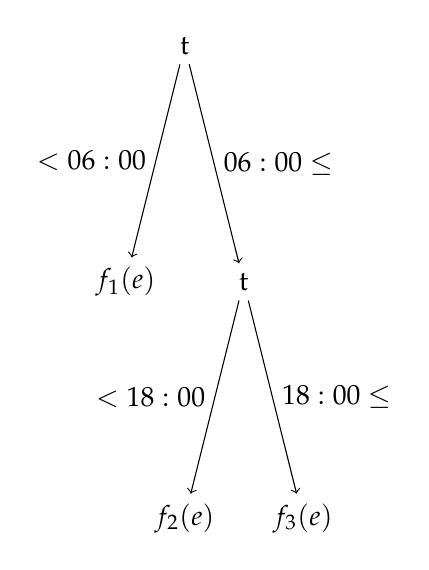
\begin{tikzpicture}
	\node {t}
	[level distance=3cm]
	child { node {$f_1(e)$} edge from parent [->] node [left] {$ < 06:00 $} }
	child { node {t}
		child { node {$f_2(e)$} edge from parent [->] node [left] {$ < 18:00 $}}
		child { node {$f_3(e)$} edge from parent [->] node [right] {$ 18:00 \le $} }
		edge from parent [->] node [right] {$06:00 \le $}
	}
	;
	\end{tikzpicture}
	\caption{Example of a simple model tree with three partitions and three linear regression models. The $t$ feature corresponds to the input time feature in equation \ref{eq:speed-piecewise}}
	\label{fig:model-tree}
\end{figure}
It works by recursively constructing a decision tree by splitting $T$ into subsets $T_1,T_2$ where the split point is determined by examining all possible splits over all non-class features and the domains of those features. The split that yields the highest reduction in standard deviation is chosen at each step.
The resulting tree is then pruned for nodes and leaves that yield a worse standard deviation reduction than parent nodes. This pruning process makes sure the final model is not overfitting the training examples and can better be applied to unseen data. 
Finally, the resulting regression models at the leaves of the tree are mutually smoothed as to minimizes sharp transitions from model to model.

Using this approach, M5' facilitates a dynamic partitioning scheme, based on the measure of standard deviation and smooths transitions between partitions.

\subsection{Generating speed functions}
% Why ?
Using the M5' implementation in Weka, we generate model trees for road segments on a day-by-day basis as described in Section \ref{traffic-patterns}. However several issues are raised about the data used for inducing the model trees:
% What ?
\begin{itemize}
\item Noisy data can skewer the regression models to be inaccurate.
\item Incorrectly mapmatched observations can skewer regression models.
\item Observed speeds above the speed limit introduces the possibility that the system can suggest driving faster than allowed.
\item A segment might not have enough observations to construct a (useful) regression model.
\end{itemize}
% How ?
To minimize the effect of these issues, we perform filtering on the observations based on the \emph{Median Sample Rate} and mapmatching error. Furthermore observations speeds higher than two times the speed limit are filtered, because such high speeds are more likely to be noise data. Observations with speeds between 100\% to 200\% the speed limit are lowered to the max speed, since such observations might be realistic, but we still do not want them to affect the regression model.

Additional thresholds for filters can be seen in \tabref{tab:datafiltering} (the green row is the one we use).
%  SELECT COUNT(o.*) FROM Observations o, Segments s, Ways w, Roadtypes t WHERE o.speed > 1 AND o.speed < t.speedlimit * 2 AND o.length > 0.005 AND o.mediansamplerate <= 20 AND o.error < 100 AND numwaypoints > 4 AND o.segment = s.id AND s.way = w.id AND w.type = t.id;
\begin{table}[H]
	\centering
	\begin{tabular}{TlTlTlTlTlTlT}
		\thickhline
		\textbf{Speed}                                                                          & \textbf{Length}  & \textbf{MSR}  & \textbf{MME} & \textbf{\#Wpts} & \textbf{Observations} \\ \thickhline
		-                                                                                       & -                & -             & -              & -               & 4584306               \\ \thickhline
		\begin{tabular}[c]{@{}l@{}}\textgreater 1 km/h\\ \textless speed limit * 2\end{tabular} & \textgreater 5 m & \textless= 20 & \textless 100  & \textgreater= 5 & 269527                \\ \thickhline
		\begin{tabular}[c]{@{}l@{}}\textgreater 1 km/h\\ \textless speed limit * 2\end{tabular} & \textgreater 5 m & \textless= 20 & \textless 100  & -               & 867128                \\ \thickhline
		\begin{tabular}[c]{@{}l@{}}\textgreater 1 km/h\\ \textless speed limit * 2\end{tabular} & -                & \textless= 20 & \textless 100  & -               & 878426                \\ \thickhline
		\textless speed limit * 2                                                               & -                & \textless= 20 & \textless 100  & -               & 898774                \\ \thickhline
		\textless= speed limit                                                                  & -                & \textless= 20 & \textless 100  & -               & 861766                \\ \thickhline
		\textless= speed limit                                                                  & -                & \textless 300 & \textless 100  & -               & 2861949               \\ \thickhline
		\rowcolor[HTML]{34FF34}
		\begin{tabular}[c]{@{}l@{}}\textgreater 1 km/h\\ \textless speed limit * 2\end{tabular} & \textgreater 5m  & \textless= 60 & \textless 100  & -               & 1715070               \\ \thickhline
		\begin{tabular}[c]{@{}l@{}}\textgreater 1 km/h\\ \textless speed limit * 2\end{tabular} & \textgreater 5m  & \textless= 60 & \textless 100  & \textgreater= 3 & 913779                \\ \thickhline
	\end{tabular}
	\caption{Observations remaining after using various filters. MSR = median sample rate of the link, \#Wpts = number of waypoints in the link.}
	\label{tab:datafiltering}
\end{table}
	\todo{make percent of how many observations (in table) are filtered. Benjamin }
\emph{MSR} is the median sample rate calculated using only waypoints that are at least 1.4 metres apart, \emph{\#Wpts} is the total number of waypoints on the link, \emph{Length} is the distance driven between the first and the last waypoint in the link, and \emph{Observations} is the number of observations remaining after applying the filters.
The tresholds are based on informal study of how high requirements of MSR and MME (mapmatching error) was possible, without discarded too much data.
Additionally, we perform normalisation of the timestamps of observations, due to Weka3's internal representation of time being problematic when doing regression.

% 	Routing approach
\section{Route planning}
\todo{How do we plan the routes? A*/D*, heuristic and cost function for capacity of roads ....}
\subsection{Contraction hierarchy}
\subsection{Cost function}
\subsection{Shortest path}
% Test, evaluation and conclusion
\chapter{Test and Evaluation}
\section{Test of client-server communication}
To be certain that our client server communication works as it should, we will do both "real-life" practical tests and black-box testing, e.g. making sure the client and server behaves as it should on different occasions.

\subsection{Connection between client and server}
To make sure that the client(s) can connect to our server we have tested it in the following ways.
\begin{itemize}
	\item From local host, we started the server from the IntelliJ IDE and afterwards we started the client from Android Studio and connected to the server. In IntelliJ we could see that the server accepted the connection. Which is shown in \figref{fig:serverrunning}.
		\begin{figure}[h!]
  \centering
	    \includegraphics[width=0.6\textwidth]{figures/serverrunning.png}
    \caption{Server running and accepting connection}
    \label{fig:serverrunning}
\end{figure}
	\item From seperate clients, we started the server as with the local host testing, but to test the targetted device, e.g smartphones, we downloaded the application to 7 smartphones and connected them to the server. It showed in IntelliJ's prompt window that the connections from each smartphone were successful.
\end{itemize}

\subsection{Message received matches the message sent}
To be certain the longitude, latitude and speed that is sent is received correctly on the server. We did the following test:
\begin{itemize}
	\item We gave the emulator in Android Studio a specific longitude and latitude and then used the application to send the data to the server. In IntelliJ's prompt window we got the following information displayed in \figref{fig:datasentfromclienttoserver}. Which confirms that the message sent from the client is received correctly on the server.
	\begin{figure}[h!]
  \centering
    \includegraphics[width=0.8\textwidth]{figures/datasentfromclienttoserver.png}
    \caption{Data received on the server from the client}
    \label{fig:datasentfromclienttoserver}
\end{figure}
	\item \todo{Use mortens phone to get a proper speed test instead of the 0.0 from the emulator}
\end{itemize}

\subsection{Is the three-way handshake condition met }
To be sure that if some message is lost or connection between the client and server is not stable, which we also described in \autoref{chap:clientserver}, we are sending acknowledgements between client server. As  \figref{fig:datasentfromclienttoserver} illustrates when the server receives data from the client the server responds with an acknowledgement message to the client, that it has received the data, the client then again responds with it's own acknowledgement message to tell the server, that it knows that the data it sent has been received.

\subsection{If server is down}
The user of the application has to be notified if they cant receive or send their data to the server. This is handled by giving a pop-up message to the user of the application that there is no connection to the server.

\subsection{GPS location and speed}
The location of the client and the speed it is moving at has been tested in a car with one person driving the car and another using a smartphone, where the smartphone displays the current speed and the location after a click on a button. The speed was compared to the car's speedometer which matched and the GPS location that was shown was later checked on a map, where the locations given by the smartphone also were correct.

\todo{Add more tests to client-server! Dont know if all of these "tests" are needed}
\section{Evaluation process}
To see how the system complies with the specified solution criteria in \secref{chap:solutioncriteria} and how the system can alleviate the problem statement, we carry out an evaluation process. More specifically, we want to evaluate the following:
% What do we look at to evaluate?
\begin{itemize}
\item How accurately does the regression models reflect the actual traffic?
\item Does the routes found based on the regression models reflect reality?
\item Are routes found by the system, based on the regression models be faster than route chosen by drivers?
\end{itemize}
% How do we evaluate?
To answer the above questions, we consider the model accuracy and time savings of the routes. 

The model accuracy is the difference between the predicted traffic of the regression model and the actual traffic. In order to find the model accuracy we consider both the accuracy on a route basis as well as on an edge basis.

Time savings represents how much faster a found route is than an actual route. This is found by comparing actual routes from a test set of routes and routes found by querying the system the same start and destination.

\subsubsection{Route evaluation}
The following method is used to find the differences between real routes driven as given by the test-set and the routes found by the system.
\begin{enumerate}
\item First, we select a route $R=(n_1,...n_m)$ from the GPS data that originates in $n_1$ and ends in $n_m$. We then, directly from the data, determine weight of the route, $W_o(R)$.
\item Secondly, we compute a new weight, $W_{a}(R)$ for every edge $(n_i,n_{i+1}) \  for \  1 \leq i \leq m$ with the weight function described in Section \ref{sec:weight-function}.
\item Now, we traverse the road network to find a new route, $R'$ originating in $n_1$ and ends in $n_m$ such that the route is the shortest path (in time) from $n_1$ to $n_m$ by using the weight of each edge determined by the weight function.
\item We compare $W_o(R)$ and $W_a(R)$ to see differeces. This is the route model accuracy.
\item Finally, we compare $W_a(R')$ with $W_a(R)$ and find the difference. This is the saved time.
\end{enumerate}
The process is illustrated in the graphs in \figref{fig:eval}. Blue nodes represent start nodes, green nodes represent goal nodes where the number in goal nodes are the aggregate weight of all the edges in the route. 

Red arrows represents the uninformed route, where the uninformed route has a weight of 7. The uninformed route with adjusted weights, has a weight of 8. This means that the regression models for the segments has an aggregate route model accuracy of $\frac{7}{8}=0.875=87.5\%$. 

By computing the informed route based on the regression model weights, the route marked with yellow arrows are found. This informed route has a lower weight than the uninformed route, which means that there can be saved time by 1.

\begin{figure}
\centering
\includegraphics[width=\textwidth]{figures/eval.pdf}
\caption{The evaluation process}
\label{fig:eval}
\end{figure}

We follow the approach on a set of 10 fairly small routes that has no signs of intermedia stops, since intermediate stops in the route, without further measuers taken, would skewer the travel time in favor of our system.

\begin{table}[H]
\centering
\begin{tabular}{llllll}
\textbf{Route} & \textbf{$W_o(R)$} & \textbf{$W_a(R)$}  & \textbf{$W_a(R')$} & \textbf{Route model accuracy (\%)} & \textbf{Time saved (\%)} \\ \hline
$r_1$          & 353               & 393                & 263                & 89.8                         & 38.5 \\
$r_2$          & 1822              & 2016               & 1552               & 90.4                         & 20.5 \\
$r_3$          & 1012              & 551                & 250                & 54.4                         & 15.3 \\
$r_4$          & 297               & 322                & 107                & 92.2                         & 43.0 \\
$r_5$          & 1248              & 927                & 797                & 74.3                         & 31.3 \\
$r_6$          & 469               & 440.5              & 440.0              & 93.9                         & 25.2 \\
$r_7$          & 1676              & 1462               & 989                & 87.2                         & 19.4 \\ \hline
mean       	   &                   &                    &                    & 83.2                         & 27.6
\end{tabular}
\caption{Model accuracy = $100 * \frac{min(W_o(R), W_a(R))}{max(W_o(R), W_a(R))}$\\
	     Time saved = $100 * \frac{W_a(R) - W_a(R')}{W_a(R)}$}
\label{tab:eval-results}
\end{table}

\tabref{tab:eval-results} shows the time in seconds, $W_0(R)$, for the uninformed route $R$, the adjusted time, $W_a(R)$, for route $R$, and the informed time $W_a(R')$ for the new (informed) route $R'$.

\textbf{Route Model accuracy} represents the difference between the uninformed weight and the adjusted weight. The closer the route model accuracy is to 100, the better the regression models represents the actual traffic.

\textbf{Time saved} represents the time saved for route $r_i$ by traveling the informed route $R'$ instead of the uninformed route $R$. The higher the time saved the better the informed routing is.

The mean route model accuracy of 71.17\%, shows that the predicted speed for a given route is within 71.17\% of the actual time it took\todo{kunne være rart at vide om det var underestimate / overestimate}. 

The mean value for time saved shows that for the tested routes, there are on average 30.661\% time saved by using the routes used by the route finding. However, it is worthwhile to note that it is not known if the drivers in the test routes was using some kind of GPS routing or not, which means that it is not possible to tell if the system outperforms routes selected by drivers or other systems.

However, the mean route model accuracy in \tabref{tab:eval-results} only shows the aggregate accuracy, which could be misleading if there is a high deviation in the regression model predictions and the actual traffic, throughout the edges. For this reason, the regression model accuracy must also be determined on an edge basis.

\subsubsection{Edge regression model}

\begin{table}[H]
	\centering
	\begin{tabular}{lll}
		\textbf{Route} & \textbf{Mean waypoints-to-waypoint error (s)}    & \textbf{Mean \%} \\ \hline
		$r_1$          & 3.66                                             & 60.2 \\
		$r_2$          & 0.722                                            & 31.9 \\
		$r_3$          & 1.61                                             & 50.0 \\
		$r_4$          & 1.69                                             & 53.6 \\
		$r_5$          & 1.13                                             & 41.0 \\
		$r_6$          & 2.70                                             & 59.1 \\
		$r_7$          & 1.01                                             & 42.1 \\ \hline
		mean           & 1.79                                             & 48.3
	\end{tabular}
	\caption{Mean \% is the mean of the percent errors of each consecutive waypoint pair.}
	\label{tab:eval-results-2}
\end{table}
\chapter{Future work}\label{ch:future-work}
\section{Future work}
\subsection{Smoothing of model tree}

\subsection{Contraction hierarchies}\label{contraction-hierarchies}
% What is it?
% Why use it?
% How do we use it?
The map is represented as a graph as this makes it a lot easier to work with path finding problems. The problem with representing a map this way is that the graph gits so big and there is a lot of unnecessary points for finding a route from A to B. To minimise the amount of data the graph consist of, shortcut have been introduce. These shortcuts are called segments, and they go from intersection to intersection, so all intermediate points on the original map is then ignored. This makes the graph a lot smaller and faster to search through.
\chapter{Conclusion}
This project presented an approach for modeling road network and traffic as weighted directed graphs with weight functions as time-based piecewise linear regression models over traffic observations of speed derived from GPS samples.

The piecewise linear regression models was found to have an average predictive accuracy of NUMBER\% of actual observed travel time on routes. This follows from several issues still present in the regression models such as limited data and improvable filtering, and could futher be improved by gathering a more useful dataset where speed is directly measured.

Furthermore the system was found to, in certain cases, be able to find alternative routes avoiding traffic congestion thus potentially provide time-savings for users of the system. By providing such a feature the system can help motorists avoid heavy traffic and be more evenly distributed on the road network.

There are many interesting areas for future work including gathering better GPS data, more accurate map-matching , optimizations in terms of utilizing advanced graph methods such as contraction hierarchies to speed up query time. Furthermore, we find it important to perform field-testing in the future, to get a much better perspective of the accuracy of the system as a whole.

To be able to collect the data needed to predict traffic patterns which our agent needs, we have constructed a client-server architecture, which is described in \ref{chap:clientserver}. The client collects data, speed, time and GPS locations, and sends that to our server where we can store the information.
\printbibliography[heading=bibintoc]
\label{bib:mybiblio}
\appendix
\input{sections/appAname.tex}
\chapter{Evaluation data}\label{app:rawevaldata}
\section*{$r_1$ data}
\textbf{Uninformed:} 353\\
\textbf{Adjusted:} 392.61656\\
\textbf{Informed:} 262.98862\\
\\
Waypoint-to-waypoint data:
\begin{longtable}{llll}
	\textbf{Actual travel time (s)} & \textbf{With adjusted weights (s)}    & \textbf{Error (s)} & \textbf{Error \%} \\ \hline
	1.0 & 1.98847 & 0.98847 & 49.71015 \\
	2.0 & 1.19308 & 0.80691 & 40.34581 \\
	5.0 & 0.39769 & 4.60230 & 92.04610 \\
	5.0 & 0.39769 & 4.60230 & 92.04610 \\
	3.0 & 2.38616 & 0.61383 & 20.46108 \\
	3.0 & 0.19884 & 2.80115 & 93.37175 \\
	5.0 & 0.19884 & 4.80115 & 96.02305 \\
	2.0 & 0.79538 & 1.20461 & 60.23054 \\
	2.0 & 0.79538 & 1.20461 & 60.23054 \\
	2.0 & 2.56780 & 0.56780 & 22.11241 \\
	2.0 & 2.56780 & 0.56780 & 22.11260 \\
	2.0 & 2.46523 & 0.46523 & 18.87184 \\
	2.0 & 2.20548 & 0.20548 & 9.31710 \\
	2.0 & 2.41395 & 0.41395 & 17.14844 \\
	2.0 & 2.36267 & 0.36267 & 15.35003 \\
	1.0 & 1.48743 & 0.48743 & 32.77001 \\
	1.0 & 1.49073 & 0.49073 & 32.91899 \\
	1.0 & 1.59001 & 0.59001 & 37.10761 \\
	1.0 & 1.59002 & 0.59002 & 37.10771 \\
	1.0 & 1.59332 & 0.59332 & 37.23811 \\
	1.0 & 1.48744 & 0.48744 & 32.77051 \\
	1.0 & 1.43945 & 0.43945 & 30.52925 \\
	1.0 & 1.48744 & 0.48744 & 32.77070 \\
	1.0 & 1.43945 & 0.43945 & 30.52945 \\
	1.0 & 1.43615 & 0.43615 & 30.36985 \\
	2.0 & 2.46529 & 0.46529 & 18.87377 \\
	2.0 & 0.99226 & 1.00773 & 50.38683 \\
	2.0 & 1.61398 & 0.38601 & 19.30082 \\
	2.0 & 2.48221 & 0.48221 & 19.42677 \\
	2.0 & 2.97834 & 0.97834 & 32.84863 \\
	2.0 & 3.22641 & 1.22641 & 38.01163 \\
	1.0 & 1.73801 & 0.73801 & 42.46315 \\
	1.0 & 1.86204 & 0.86204 & 46.29574 \\
	1.0 & 1.98608 & 0.98608 & 49.64963 \\
	1.0 & 1.98608 & 0.98608 & 49.64963 \\
	1.0 & 2.23414 & 1.23414 & 55.24022 \\
	1.0 & 2.10856 & 1.10856 & 52.57427 \\
	1.0 & 2.11011 & 1.11011 & 52.60924 \\
	1.0 & 2.23414 & 1.23414 & 55.24023 \\
	1.0 & 2.11011 & 1.11011 & 52.60924 \\
	1.0 & 2.23414 & 1.23414 & 55.24023 \\
	1.0 & 2.23414 & 1.23414 & 55.24023 \\
	1.0 & 2.23414 & 1.23414 & 55.24024 \\
	1.0 & 2.48221 & 1.48221 & 59.71341 \\
	1.0 & 2.35818 & 1.35818 & 57.59446 \\
	1.0 & 2.35818 & 1.35818 & 57.59446 \\
	1.0 & 2.23415 & 1.23415 & 55.24024 \\
	1.0 & 2.23415 & 1.23415 & 55.24025 \\
	1.0 & 1.73801 & 0.73801 & 42.46320 \\
	2.0 & 2.48221 & 0.48221 & 19.42684 \\
	5.0 & 1.11632 & 3.88367 & 77.67340 \\
	5.0 & 145.17850 & 140.17850 & 96.55596 \\
	5.0 & 0.49613 & 4.50386 & 90.07735 \\
	5.0 & 0.24962 & 4.75037 & 95.00756 \\
	5.0 & 0.12558 & 4.87441 & 97.48822 \\
	5.0 & 0.99226 & 4.00773 & 80.15471 \\
	2.0 & 1.61403 & 0.38596 & 19.29825 \\
	2.0 & 2.56245 & 0.56245 & 21.94984 \\
	2.0 & 3.70050 & 1.70050 & 45.95336 \\
	1.0 & 1.85117 & 0.85117 & 45.98016 \\
	1.0 & 2.13384 & 1.13384 & 53.13633 \\
	1.0 & 2.27794 & 1.27794 & 56.10072 \\
	1.0 & 2.27794 & 1.27794 & 56.10072 \\
	1.0 & 2.56245 & 1.56245 & 60.97493 \\
	1.0 & 2.70471 & 1.70471 & 63.02748 \\
	1.0 & 2.56245 & 1.56245 & 60.97493 \\
	1.0 & 2.70471 & 1.70471 & 63.02749 \\
	1.0 & 2.84696 & 1.84696 & 64.87492 \\
	1.0 & 2.84696 & 1.84696 & 64.87492 \\
	1.0 & 2.98922 & 1.98922 & 66.54652 \\
	1.0 & 3.13148 & 2.13148 & 68.06624 \\
	1.0 & 2.98922 & 1.98922 & 66.54653 \\
	1.0 & 3.27374 & 2.27374 & 69.45389 \\
	1.0 & 3.13148 & 2.13148 & 68.06625 \\
	1.0 & 3.13148 & 2.13148 & 68.06625 \\
	1.0 & 3.13331 & 2.13331 & 68.08496 \\
	1.0 & 2.98922 & 1.98922 & 66.54654 \\
	1.0 & 2.98922 & 1.98922 & 66.54654 \\
	1.0 & 2.70471 & 1.70471 & 63.02751 \\
	1.0 & 2.70471 & 1.70471 & 63.02751 \\
	1.0 & 2.56245 & 1.56245 & 60.97496 \\
	1.0 & 2.56062 & 1.56062 & 60.94699 \\
	1.0 & 2.42020 & 1.42020 & 58.68112 \\
	1.0 & 2.56245 & 1.56245 & 60.97497 \\
	1.0 & 2.27794 & 1.27794 & 56.10077 \\
	1.0 & 2.13568 & 1.13568 & 53.17667 \\
	1.0 & 1.99343 & 0.99343 & 49.83523 \\
	1.0 & 1.99159 & 0.99159 & 49.78899 \\
	2.0 & 2.84697 & 0.84697 & 29.74992 \\
	3.0 & 2.13568 & 0.86431 & 28.81039 \\
	5.0 & 0.71128 & 4.28871 & 85.77431 \\
	3.0 & 0.0 & 3.0 & 100.0 \\
	2.0 & 0.0 & 2.0 & 100.0 \\
	5.0 & 0.99763 & 4.00236 & 80.04732 \\
	3.0 & 2.84697 & 0.15302 & 5.10091 \\
	2.0 & 2.70471 & 0.70471 & 26.05507 \\
	1.0 & 0.0 & 1.0 & 100.0 \\
	1.0 & 0.0 & 1.0 & 100.0 \\
	1.0 & 0.0 & 1.0 & 100.0 \\
	1.0 & 0.0 & 1.0 & 100.0 \\
	1.0 & 0.0 & 1.0 & 100.0 \\
	3.0 & 91.78741 & 88.78741 & 96.73157 \\
	3.0 & 2.20435 & 0.79564 & 26.52151 \\
	3.0 & 2.34260 & 0.65739 & 21.91327 \\
	3.0 & 2.06658 & 0.93341 & 31.11392 \\
	1.0 & 2.20435 & 1.20435 & 54.63524 \\
	2.0 & 2.06658 & 0.06658 & 3.22185 \\
	4.0 & 0.96440 & 3.03559 & 75.88987 \\
	4.0 & 0.0 & 4.0 & 100.0 \\
	4.0 & 0.27554 & 3.72445 & 93.11139 \\
	5.0 & 0.41331 & 4.58668 & 91.73367 \\
	5.0 & 0.0 & 5.0 & 100.0 \\
	5.0 & 0.0 & 5.0 & 100.0 \\
	5.0 & 0.0 & 5.0 & 100.0 \\
	3.0 & 0.0 & 3.0 & 100.0 \\
	2.0 & 0.13777 & 1.86222 & 93.11139 \\
	5.0 & 0.0 & 5.0 & 100.0 \\
	5.0 & 0.27554 & 4.72445 & 94.48911 \\
	5.0 & 0.41331 & 4.58668 & 91.73367 \\
	5.0 & 0.68886 & 4.31113 & 86.22278 \\
	5.0 & 0.82710 & 4.17289 & 83.45783 \\
	5.0 & 1.23994 & 3.76005 & 75.20101 \\
	5.0 & 0.68886 & 4.31113 & 86.22278 \\
	5.0 & 1.23994 & 3.76005 & 75.20101 \\
	5.0 & 0.0 & 5.0 & 100.0 \\
	5.0 & 0.27554 & 4.72445 & 94.48911 \\
	5.0 & 0.55108 & 4.44891 & 88.97822 \\
	5.0 & 0.27554 & 4.72445 & 94.48911 \\ \hline
	& mean & 3.66470 & 60.18249 \\
  & median & 1.63358 & 62.00121
\end{longtable}

\section*{$r_1$ data}
\textbf{Uninformed:} 1\\
\textbf{Adjusted:} 2\\
\textbf{Informed:} 3\\
\\
Waypoint-to-waypoint data:
\begin{longtable}{llll}
	\textbf{Actual travel time (s)} & \textbf{With adjusted weights (s)}    & \textbf{Error (s)} & \textbf{Error \%} \\ \hline
	a & b & c & d \\ \hline
	& mean & e & f \\
	& median & g & h
\end{longtable}

\input{sections/nicefigureApp.tex}
\end{document}